Konflikte werden in beiden Prototypen manuell erzeugt, wobei die Vorgehensweise identisch ist.
Wie ein Konflikt herbeigeführt werden kann, wird in \autoref{chap:konzept:test} beschrieben.
Durch das regelmäßige Anfragen an den Server wird dargestellt, ob sich die Anwendung im Onlinestatus befindet oder nicht.
Konflikte können erzeugt werden, wenn ein oder beide Geräte auf denen die Anwendung läuft nicht mit dem Internet verbunden ist.
Die Anzeige im Header dient der Kontrolle über diesen Status.
Die folgenden Codeausschnitte illustrieren das Konfliktmanagement im Prototypen \it{amilia-qouch}.\\
Konflikte werden in CouchDB gespeichert, damit in der Anwendung entschieden werden kann wie damit umgegangen wird.
Im \autoref{code:conflicts} werden alle Kontakteinträge geladen.
Weil der Parameter in Zeile 3 als Option mitgegeben wird, sind Konfliktinformationen für jeden Kontakt verfügbar.
Gibt es unterschiedliche Versionen eines Kontaktes kommt er mit dem Attribut \tt{\_conflicts} beim Client an, und zwar in Form eine Liste aus allen korrelierenden Revisionsnummern.
In Zeile 7 wird der erste konfliktbehaftete Kontakt, der vom Server kommt, ermittelt.
Wenn es einen Konflikt gibt, wird die Funktion \tt{getConflictRevisions} in Zeile 10 aufgerufen.
%
\begin{center}
  \lstinputlisting[language=REACT,
    firstline=1,lastline=12,
    numbers=left,xleftmargin=20pt,framexleftmargin=15pt,
    caption={Das Laden von konfliktbehafteten Kontakten},
    label=code:conflicts]{code/conflicts.js}
\end{center}
%
\autoref{code:conflicts2} zeigt die Umsetzung der \tt{getConflictRevisions()}.
Hier wird die konkurrierende Version des Kontakts ermittelt.
Außerdem wird die Herkunft jeder Version festgestellt und das Öffnen eines Konfliktdialogs eingeleitet.\\
In Zeile 2 werden die Variablen \tt{contactMe} und \tt{contactYou} initialisiert.
Die erste repräsentiert die lokale Version, \tt{contactYou} steht für die Version die aus der CouchDB kommt.
In Zeile 4 wird überprüft, ob die übergebene Version des Kontakts mit der zuletzt bearbeiteten übereinstimmt.
Entsprechend werden die Variablen \tt{contactMe} und \tt{contactYou} befüllt.
Die übergebene Version ist die von CouchDB festgelegte gewinnende Revision.
Die andere, konkurrierende Version wird in Zeile 8, bzw. in Zeile 13 durch die Übergabe der Revisionsnummer im Parameter geladen.
Die ID ist bei beiden Versionen identisch.\\
%
Dann wird das Öffnen des Konfliktdialogs durch das Aktualisieren des \gls{App}status initialisiert.
Die beiden Kontaktversionen werden ebenfalls in den State geladen, um im Dialog korrekt angezeigt zu werden.
%
\begin{center}
  \lstinputlisting[language=REACT,
    firstline=14,lastline=38,
    numbers=left,xleftmargin=20pt,framexleftmargin=15pt,
    caption={Das Ermitteln von konkurrierenden Kontaktversionen},
    label=code:conflicts2]{code/conflicts.js}
\end{center}
%
Der Konfliktdialog ist in \autoref{fig:modal} dargestellt.
Im Titel steht der Name der lokalen Version, rot hervorgehoben.
Darunter befinden sich zwei große Knöpfe in unterschiedlichen Farben.
Der erste zeigt die Version des Kontakts, die vom Server kommt, die auf einem anderen Gerät bearbeitet wurde.
Der zweite, untere Knopf beinhaltet alle relevanten Informationen über die lokale Version des konfliktbehafteten Kontakts.
So ist zu erkennen welche der beiden Versionen die eigene ist und worin sie sich von der anderen unterscheidet.
%
\begin{figure}[H]
  \centering
  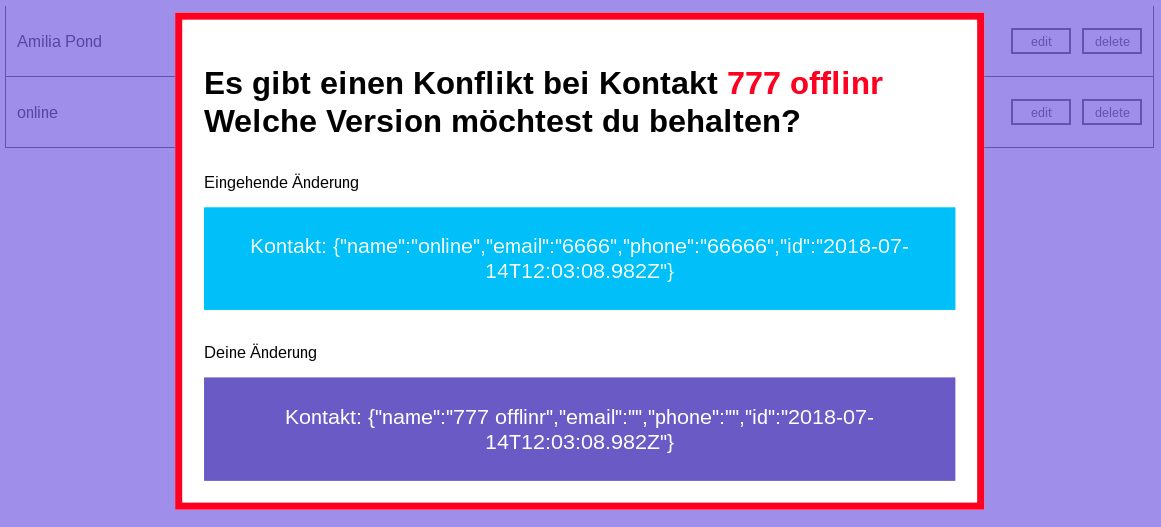
\includegraphics[width=\textwidth]{impl/Modal}
  \grayRule
  \caption{Konfliktdialog des Prototypen amilia-qouch}
  \label{fig:modal}
\end{figure}
%
Durch das Klicken einer dieser Knöpfe wird entschieden, welche der beiden Versionen behalten und welche eliminiert wird.
Wird der Knopf mit der lokalen Version betätigt, wird die in \autoref{code:conflicts3} gelistete Funktion \tt{removeRev} mit der anderen Version im Parameter aufgerufen.
%
\begin{center}
  \lstinputlisting[language=REACT,
    firstline=40,lastline=43,
    numbers=left,xleftmargin=20pt,framexleftmargin=15pt,
    caption={Das Eliminieren der verlierenden Version},
    label=code:conflicts3]{code/conflicts.js}
\end{center}
%
Dort, in Zeile drei, wird die verlierende Revision gelöscht.\\\\
%
%
Der Konfliktdialog konnte für den Protoypen \it{amilia-rdx} nicht umgesetzt werden, da Redux offline nicht die Möglichkeit bietet Konflikte zu erkennen, geschweige denn zu speichern.